
\[
\vec g (\vec r) = -\vec\nabla U (\vec r)
\]
with 
\[
U(\vec r) = {\cal G} \int\int\int \frac{\rho(\vec r')}{|\vec r-\vec r'|}dV
\]
with (in a Cartesian coordinates system):
\[
|\vec r-\vec r'|=\sqrt{(x-x')^2 + (y-y')^2 + (z-z')^2}
\qquad dV = dx'dy'dz'
\]
We then have 
\begin{eqnarray}
g_x (x,y,z) 
&=& - {\cal G} \int\int\int \frac{\partial }{\partial x} \frac{\rho(\vec r')}{|\vec r-\vec r'|}dx'dy'dz' \nn\\
&=&  {\cal G} \int\int\int \frac{\rho(\vec r') (x-x')}{|\vec r-\vec r'|^3}dx'dy'dz' \nn\\
g_y (x,y,z) 
&=& - {\cal G} \int\int\int \frac{\partial }{\partial y} \frac{\rho(\vec r')}{|\vec r-\vec r'|}dx'dy'dz' \nn\\
&=&  {\cal G} \int\int\int \frac{\rho(\vec r') (y-y')}{|\vec r-\vec r'|^3}dx'dy'dz' \nn\\
g_z (x,y,z) 
&=& - {\cal G} \int\int\int \frac{\partial }{\partial z} \frac{\rho(\vec r')}{|\vec r-\vec r'|}dx'dy'dz' \nn\\
&=&  {\cal G} \int\int\int \frac{\rho(\vec r') (z-z')}{|\vec r-\vec r'|^3}dx'dy'dz' \nn
\end{eqnarray}

\index{general}{Marussi Tensor}
In order to compute the gravity tensor ${\bm T}=\vec\nabla \vec g$, also called gravitational gravity tensor \cite{ruys11}
or Marussi tensor,  
we need to compute $\frac{\partial^2 U}{\partial \alpha \partial \beta}$ with $\alpha,\beta=x,y,z$
and we obtain (See Arroyo \etal (2015) \cite{arct15}):
\begin{eqnarray}
T_{xx}(x,y,z)&=& -{\cal G} \int\int\int \frac{3(x-x')^2-({\vec r}-{\vec r}')^2}{|{\vec r}-{\vec r}'|^5} \rho({\vec r}') dx'dy'dz' \\
T_{yy}(x,y,z)&=& -{\cal G} \int\int\int \frac{3(y-y')^2-({\vec r}-{\vec r}')^2}{|{\vec r}-{\vec r}'|^5} \rho({\vec r}') dx'dy'dz' \\
T_{zz}(x,y,z)&=& -{\cal G} \int\int\int \frac{3(z-z')^2-({\vec r}-{\vec r}')^2}{|{\vec r}-{\vec r}'|^5} \rho({\vec r}') dx'dy'dz' \\
T_{xy}(x,y,z)&=& -{\cal G} \int\int\int \frac{3(x-x')(y-y')}{|{\vec r}-{\vec r}'|^5}  \rho({\vec r}') dx'dy'dz' \\
T_{xz}(x,y,z)&=& -{\cal G} \int\int\int \frac{3(x-x')(z-z')}{|{\vec r}-{\vec r}'|^5}  \rho({\vec r}') dx'dy'dz' \\
T_{yz}(x,y,z)&=& -{\cal G} \int\int\int \frac{3(y-y')(z-z')}{|{\vec r}-{\vec r}'|^5}  \rho({\vec r}') dx'dy'dz' 
\end{eqnarray}
Note that the trace satisfies the Laplace equation $T_{xx}+T_{yy}+T_{zz}=\Delta U = 0$.

\todo[inline]{redo all calculations to be sure}

Unless the geometry is conveniently chosen with lots of symmetry and the density is also very simple the above 
integrals cannot be computed analyticaly and one must resort to numerical integration based on a tesselation of the 
space, such as prisms or tesseroids. 

%........................
\subsubsection{Prisms}

\index{general}{Prism}

The gravitational potential $U$ of a right rectangular parallelopiped (prism) of homogeneous mass-density $\rho_0$ is
described by Newton's integral \cite{hese07}
\[
U(x,y,z) 
= {\cal G} \rho_0 \int_{z_1}^{z_2}\int_{y_1}^{y_2}\int_{x_1}^{x_2} \frac{1}{|\vec r-\vec r'|}dx'dy'dz'
= {\cal G} \rho_0 \int_{z_1}^{z_2}\int_{y_1}^{y_2}\int_{x_1}^{x_2} \frac{1}{\sqrt{(x-x')^2+(y-y')^2+(z-z')^2} }dx'dy'dz'
\]

\begin{center}
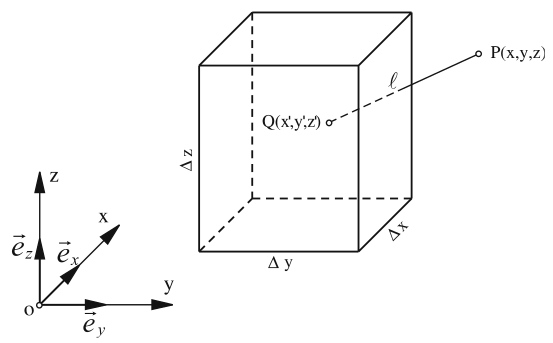
\includegraphics[width=5cm]{images/gravity/hese07}\\
{\captionfont Taken from \cite{hese07}.}
\end{center}

The denominator is the distance between the computation point $P(x,y,z)$ 
and the running integration point $Q(x',y',z')$. 
The coordinate axes have been assumed to be parallel to the edges of the prism, which
extends between the coordinate surfaces related to the
bounds $x_1$, $x_2$, $y_1$, $y_2$, $z_1$, $z_2$.
It is well known that the integral can be solved analytically (Mader (1951) \cite{made51}, 
see also Nagy \etal \cite{napb00,napb02}), 
resulting in the formula for the potential $U(x,y,z)$:

\[
U(x,y,z)= {\cal G} \rho_0
\sum_{i=1}^2\sum_{j=1}^2\sum_{k=1}^2 (-1)^{i+j+k}
\left(A+B+C-\frac{1}{2}D\right)
\]
with 
\begin{eqnarray}
A&=& (x-x_i)(y-y_j) \ln \left|  \frac{z-z_k + r_{ijk}}{\sqrt{(x-x_i)^2+(y-y_j)^2}}   \right| \nn\\
B&=& (y-y_j)(z-z_j) \ln \left|  \frac{x-x_i + r_{ijk}}{\sqrt{(y-y_j)^2+(z-z_k)^2}}   \right| \nn\\
C&=& (x-x_i)(z-z_k) \ln \left|  \frac{y-y_j + r_{ijk}}{\sqrt{(z-z_k)^2+(x-x_i)^2}}   \right| \nn\\
D&=& (x-x_i)^2 \arctan \frac{(y-y_j) (z-z_k)}{(x-x_i) r_{ijk}} \nn\\
 &+& (y-y_j)^2 \arctan \frac{(z-z_k) (x-x_i)}{(y-y_j) r_{ijk}} \nn\\
 &+& (z-z_k)^2 \arctan \frac{(x-x_i) (y-y_j)}{(z-z_k) r_{ijk}} \nn 
\end{eqnarray}
and 
\[
r_{ijk}=\sqrt{ (x-x_i)^2+(y-y_j)^2+(z-z_k)^2}
\]
\begin{remark}
The direct application of this equation will fail when the computation point $P$ is situated on an edge or on
a corner of the prism; the respective limit values have been derived by Nagy \etal \cite{napb00,napb02}
\end{remark}


The gravity vector and tensor can then be computed \cite{plou76,arct15,cooo15}:
\begin{eqnarray}
g_x(x,y,z) &=&{\cal G} \rho_0 \sum_{i=1}^2\sum_{j=1}^2\sum_{k=1}^2 (-1)^{i+j+k} \times \nn\\
&&\left[(y-y_j) \ln((z-z_k)+r_{ijk}) + (z-z_k)\ln((y-y_j)+r_{ijk}) - (x-x_i) \arctan  \frac{(y-y_j( (z-z_k)}{(x-x_i) r_{ijk}} \right] \nn\\ 
g_y(x,y,z) &=&{\cal G} \rho_0 \sum_{i=1}^2\sum_{j=1}^2\sum_{k=1}^2 (-1)^{i+j+k} \times \nn\\
&&\left[(z-z_k) \ln((x-x_i)+r_{ijk}) + (x-x_i)\ln((z-z_k)+r_{ijk}) - (y-y_j) \arctan  \frac{(x-x_i) (z-z_k)}{(y-y_j) r_{ijk}} \right] \nn\\ 
g_z(x,y,z) &=&{\cal G} \rho_0 \sum_{i=1}^2\sum_{j=1}^2\sum_{k=1}^2 (-1)^{i+j+k} \times \nn\\
&&\left[(y-y_j) \ln((x-x_i)+r_{ijk}) + (x-x_i)\ln((y-y_j)+r_{ijk}) - (z-z_k) \arctan  \frac{(x-x_i) (y-y_j)}{(z-z_k) r_{ijk}} \right] \nn\\ 
T_{xx}(x,y,z) &=& {\cal G} \rho_0 \sum_{i=1}^2\sum_{j=1}^2\sum_{k=1}^2 (-1)^{i+j+k} \arctan \frac{(y-y_j) (z-z_k)}{(x-x_i) r_{ijk}}\nn\\
T_{yy}(x,y,z) &=& {\cal G} \rho_0 \sum_{i=1}^2\sum_{j=1}^2\sum_{k=1}^2 (-1)^{i+j+k} \arctan \frac{(x-x_i) (z-z_k)}{(y-y_j) r_{ijk}}\nn\\
T_{zz}(x,y,z) &=& {\cal G} \rho_0 \sum_{i=1}^2\sum_{j=1}^2\sum_{k=1}^2 (-1)^{i+j+k} \arctan \frac{(x-x_i) (y-y_j)}{(z-z_k) r_{ijk}}\nn\\
T_{xy}(x,y,z) &=& {\cal G} \rho_0 \sum_{i=1}^2\sum_{j=1}^2\sum_{k=1}^2 (-1)^{i+j+k} \ln ((z-z_k) + r_{ijk})\nn\\
T_{xz}(x,y,z) &=& {\cal G} \rho_0 \sum_{i=1}^2\sum_{j=1}^2\sum_{k=1}^2 (-1)^{i+j+k} \ln ((y-y_j) + r_{ijk})\nn\\
T_{yz}(x,y,z) &=& {\cal G} \rho_0 \sum_{i=1}^2\sum_{j=1}^2\sum_{k=1}^2 (-1)^{i+j+k} \ln ((x-x_i) + r_{ijk})\nn
\end{eqnarray}

Note that Heck \& Seitz \cite{hese07} report that the logarithmic terms can be transformed in order to provide a better numerical stability and then

\begin{eqnarray}
g_x(x,y,z) 
&=&{\cal G} \rho_0 \sum_{i=1}^2\sum_{j=1}^2\sum_{k=1}^2 (-1)^{i+j+k}  
\left[(y-y_j) \ln \left|\frac{(z-z_k)+r_{ijk}}{\sqrt{(x-x_i}^2+(y-y_j)^2}\right|   \right. \nn\\
&& \left.  + (z-z_k) \ln \left| \frac{ (y-y_j)+r_{ijk}}{ \sqrt{(x-x_i}^2+(z-z_k)^2 } \right|
  - (x-x_i) \arctan  \frac{(y-y_j) (z-z_k)}{(x-x_i) r_{ijk}} \right] 
\end{eqnarray}

The gravitational potential of the homogeneous rectangular prism, 
neglecting terms of order four and higher in $x$, $y$, $z$, 
is then given by MacMillan's (1930)\footnote{MacMillan WD (1930) Theoretical Mechanics, vol 2: the The-
ory of the potential. McGraw-Hill, New York (reprinted by Dover Publications, New York 1958)} formula:
\[
U(x,y,z) = {\cal G} \rho_0 \Delta_x \Delta_y \Delta_y
\left[
\frac{1}{l_0}
+ \frac{3(x_0-x)^2-l_0^2}{24l_0^5}\Delta_x^2
+ \frac{3(y-y_0)^2-l_0^2}{24l_0^5}\Delta_y^2
+ \frac{3(z-z_0)^2-l_0^2}{24l_0^5}\Delta_z^2
+ {\cal O}(\Delta^4)
\right]
\]

\begin{center}
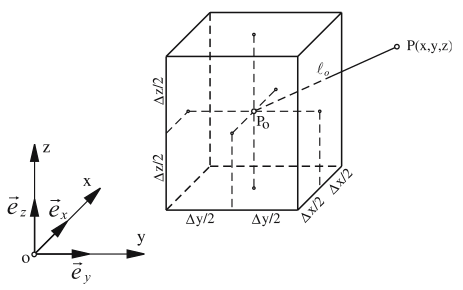
\includegraphics[width=5cm]{images/gravity/hese07b}\\
{\captionfont Taken from \cite{hese07}.}
\end{center}

It is obvious that the zero-order approximation is 
identical with the potential of a point-mass at $P_0$ 
when the total mass of the prism $m=\rho_0 \Delta_x \Delta_y \Delta_z$ 
is concentrated at its geometrical centre $P_0$:
\[
U(x,y,z) = {\cal G} \rho_0 \Delta_x \Delta_y \Delta_y \frac{1}{l_0}
\]

It is also common \cite{duti16} to look at:
\begin{itemize}
\index{general}{Differential Curvature Magnitude}
\item the differential curvature magnitude ($DCM$) 
which is also known as the horizontal directive tendency, computed by a
combination of components of tensor $T_{xx}$ , $T_{xy}$ and $T_{yy}$ . 
It emphasizes greatly the effects of shallower sources (Saad, 2006);
\[
DCM=\sqrt{ (T_{xx}-T_{yy})^2+ 2 T_{xy}^2 }
\]
\index{general}{Horizontal Gradient Magnitude}
\item the horizontal gradient magnitude ($HGM$) of $g_z$ can be computed
from the horizontal derivative components of $g_z$ and can be used
as edge detector or to map the body outline as it verifies the prism
boundaries
\[
HGM=\sqrt{T_{zx}^2+T_{zy}^2} 
=\sqrt{ \left(-\frac{\partial g_z}{\partial x}\right)^2 
+ \left(-\frac{\partial g_z}{\partial y}\right)^2  }
\]

\index{general}{Total Gradient Magnitude}
\item the total gradient magnitude ($TGM$) is
computed from the three derivatives of vertical component of gravity:
\[
TGM=\sqrt{T_{zx}^2+T_{zy}^2+T_{zz}^2}
=\sqrt{ \left(-\frac{\partial g_z}{\partial x}\right)^2 
+ \left(-\frac{\partial g_z}{\partial y}\right)^2  
+ \left(-\frac{\partial g_z}{\partial z}\right)^2  }
\]

\end{itemize}

\newpage
\paragraph{Example 1}
The result of calculating
the components of a prism measuring 200m$^3$ at a height of 0.01 km, 
with an observation mesh of 1km$\times$1km, and discretized every 20m is shown hereunder:
\begin{center}
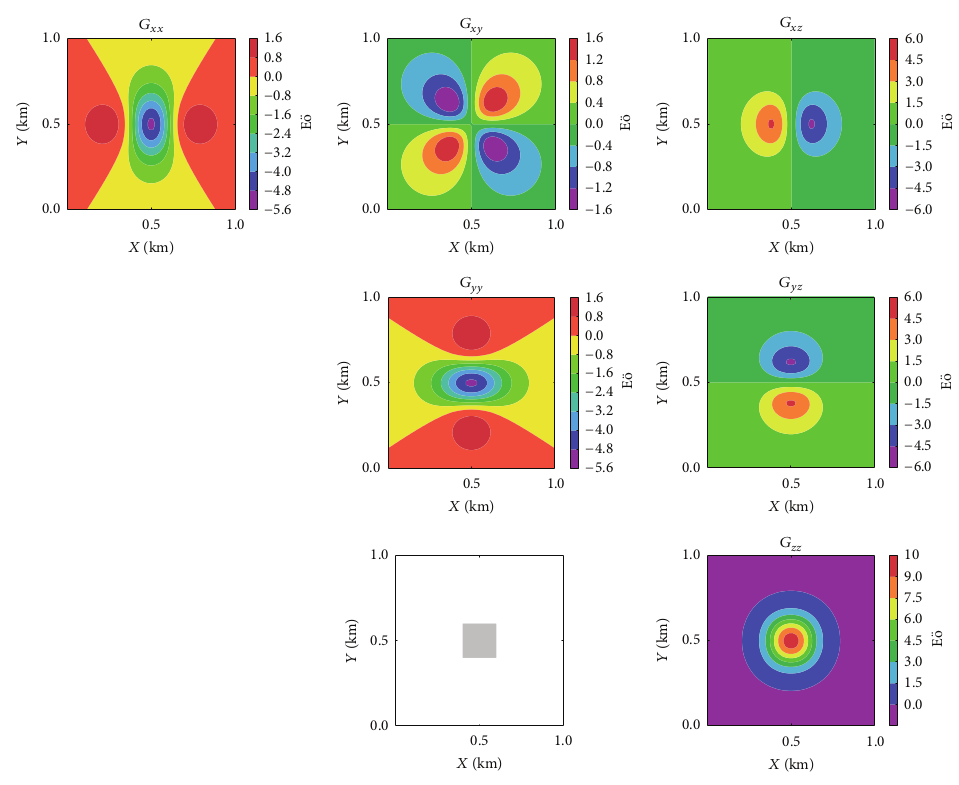
\includegraphics[width=14cm]{images/gravity/arct15b}\\
{\captionfont Taken from Arroyo \etal (2015) \cite{arct15}. 
Gravity gradient response for a prism buried a depth of 100m,\\ 
Each side having a length of 200 m and constant density contrast 
of 100 kg/m$^3$.}
\end{center}


\newpage
\paragraph{Example 2}. Buried prims of size 8x4x1 km along x, y and z directions respectively. 
Density is 2700. Mapped gravity field and its gradient on a plane of constant 1000m height.

\begin{center}
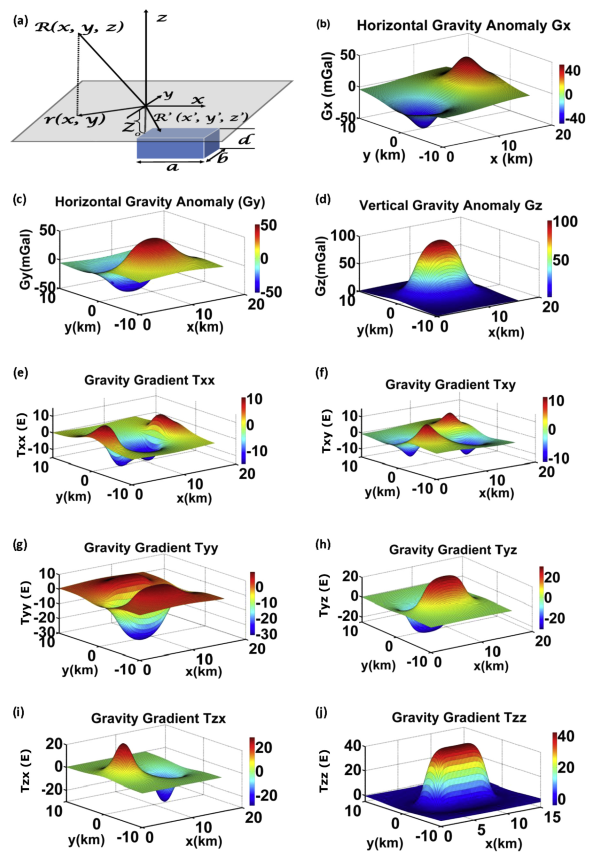
\includegraphics[width=13cm]{images/gravity/duti16a}\\
{\captionfont (a) A model containing a prism and (b-d): corresponding gravity vector components and 
(e-j) GGT components with sampling interval of 0.2 km in x and y directions. Taken from \cite{duti16}}
\end{center}

\begin{center}
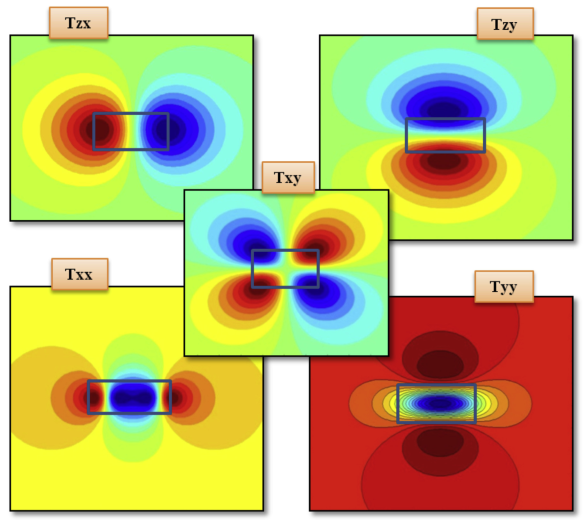
\includegraphics[width=13cm]{images/gravity/duti16b}\\
{\captionfont A map view of complex behavior of gravity gradients for prism model. Taken from \cite{duti16}}
\end{center}

\begin{center}
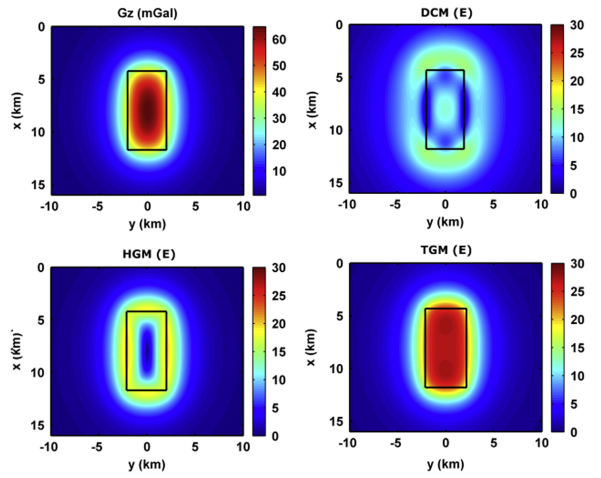
\includegraphics[width=13cm]{images/gravity/duti16c}\\
{\captionfont Computed vertical gravity component G z and three invariants map of HGM, DCM and TGM 
for given prism model. HGM = Horizontal Gradient Magnitude,
DCM = Differential Curvature Magnitude and TGM = Total Gradient Magnitude. Taken from \cite{duti16}}
\end{center}







\Literature:
\begin{itemize}
\item Analytic Expressions for the Gravity Gradient Tensor 
      of 3D Prisms with Depth-Dependent Density \cite{jilz18}
\item New computationally efficient quadrature formulas for triangular prism elements \cite{kuym13}
\item 3D Gravity Modeling of Complex Salt Features in the Southern Gulf of Mexico \cite{naoo16}.
\item Spherical prism gravity effects by Gauss-Legendre quadrature integration \cite{asvk07}
\item Perturbing effects of sub-lithospheric mass anomalies in GOCE gravity gradient and other 
      gravity data modelling: Application to the Atlantic-Mediterranean transition zone \cite{furc15}
\end{itemize}

\bscthesis \index{general}{BSc Thesis} Sort out the mess by \cite{duti16} and \cite{zhhu17}.



%.........................
\subsubsection{Tesseroids}

A tesseroid, or spherical prism, is segment of a sphere. 

\index{general}{Tesseroid}

\begin{center}
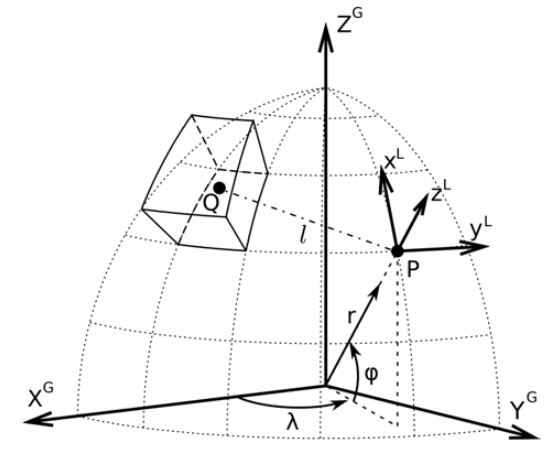
\includegraphics[width=7cm]{images/gravity/uibb11}\\
{\captionfont Taken from \cite{uibb11}}
\end{center}

Tesseroids is a collection of command-line programs for modeling the gravitational potential, 
acceleration, and gradient tensor. Tesseroids supports models and computation grids 
in Cartesian and spherical coordinates.
\url{https://tesseroids.readthedocs.io/en/stable/}

\Literature:
\begin{itemize}
\item Forward modeling and inversion of gravitational fields in spherical coordinates, L. Uieda, Phd Thesis 
\cite{uied16}
\item Tesseroids: Forward-modeling gravitational fields in spherical coordinates \cite{uibb15}
\item Optimal forward calculation method of the Marussi tensor due to a geologic structure at GOCE height 
\cite{uibb11}
\item Optimized formulas for the gravitational field of a tesseroid \cite{grsh13}
\end{itemize}



%.........................
\subsubsection{Tetrahedra}

See Werner \& Scheeres (1997) \cite{wesc97}



%.........................
\subsubsection{Other shapes}

\Literature

Rapid Gravity Computations for Two-Dimensional Bodies \cite{tawl59}

Rapid Computation of Gravitational Attraction of Three-Dimensional Bodies of Arbitrary Shape
\cite{taew60}




